\documentclass[11pt]{article}
\usepackage[textwidth=15cm,textheight=22cm]{geometry}
\usepackage{amsmath,amssymb,amsthm,booktabs,graphicx,array}
\usepackage[colorlinks=true,linkcolor=blue,citecolor=blue,urlcolor=blue]{hyperref}
\setlength{\emergencystretch}{2.5em}
\newtheorem*{proposition5}{Proposition 5}\newtheorem*{proposition6}{Proposition 6}\newtheorem*{theorem7}{Theorem 7}
\renewcommand{\thetable}{S\arabic{table}}\renewcommand{\thefigure}{S\arabic{figure}}
\title{Supplementary Material for\\ ``Real spectra and fast tensor solvers for midpoint quadratic-spline collocation on graded grids''}
\author{Farshid Mossaiby}
\date{}
\begin{document}
\maketitle
\noindent Theorem, corollary and proposition numbers refer to the main article. Part~A proves
Propositions~5 and~6 and Theorem~7; the proofs of Theorem~1, Corollary~2 and Theorem~3 are in the appendix of
the article. Part~B contains additional tables and a figure, all generated by the scripts of the repository
\url{https://github.com/mossaiby/iHaar} (release v1.1).

\section*{Part A. Proofs of Propositions 5 and 6 and Theorem 7}
\subsection*{Notation}
The grid is $a=t_0<\dots<t_N=b$, with cells $I_k$ of width $h_k$, midpoints $m_k$ and midpoint spacings
$d_k=(h_k+h_{k+1})/2$; $U_k$ are the nodal values and $c_k$ the cell values of $s''$. The three-term identity
(Theorem~1) reads, in the interior and at a zero-slope or prescribed-value left end,
\begin{equation}\label{eq:interior}
\frac{U_{k+1}-U_k}{d_k}-\frac{U_k-U_{k-1}}{d_{k-1}}
=\frac{h_{k-1}^2}{8d_{k-1}}c_{k-1}+\Big(h_k-\frac{h_k^2}{8d_{k-1}}-\frac{h_k^2}{8d_k}\Big)c_k+\frac{h_{k+1}^2}{8d_k}c_{k+1}.
\end{equation}
At the left end, with $g_0=s(a)$,
\begin{align}
\frac{U_2-U_1}{d_1}-\frac{2(U_1-g_0)}{h_1}&=\Big(\frac{3h_1}{4}-\frac{h_1^2}{8d_1}\Big)c_1+\frac{h_2^2}{8d_1}c_2 ,\label{eq:dirrow}\\
\frac{U_2-U_1}{d_1}&=\Big(h_1-\frac{h_1^2}{8d_1}\Big)c_1+\frac{h_2^2}{8d_1}c_2 ,\label{eq:neurow}
\end{align}

For the phase-field schemes on a uniform grid, $K=-\Delta_h$ is the negative of the tensor-sum discrete
Laplacian built from $D_2$ or $D_2^{(4)}$, $\langle v,w\rangle_h=h^d\sum vw$,
$E_{1,h}(u)=\langle\frac14(u^2-1)^2,1\rangle_h$, $f(u)=u^3-u$, $G_h=I$ (Allen--Cahn) or $G_h=K$
(Cahn--Hilliard), $\bar u=2u^n-u^{n-1}$, $\bar b=f(\bar u)/\sqrt{E_{1,h}(\bar u)+C}$ with $C>0$, and $S\ge0$.
The stabilized SAV-BDF2 scheme is
\begin{align}
\frac{3u^{n+1}-4u^n+u^{n-1}}{2\Delta t}&=-G_h\mu^{n+1},\qquad
\mu^{n+1}=\varepsilon^2Ku^{n+1}+S(u^{n+1}-\bar u)+r^{n+1}\bar b,\label{eq:sav1}\\
3r^{n+1}-4r^n+r^{n-1}&=\tfrac12\langle\bar b,3u^{n+1}-4u^n+u^{n-1}\rangle_h,\label{eq:sav2}
\end{align}

\subsection*{Statements}
\begin{proposition5}[Uniform grids]
On a uniform grid, \begin{equation}\label{eq:D2}D_2=\frac{8}{h^2}\delta^2(8I+\delta^2)^{-1},\end{equation}, where $\delta^2$ is the three-point second
difference with end entries $-3$ (prescribed value) or $-1$ (zero slope). It is symmetric and diagonalized
by the discrete sine (prescribed values) or cosine (zero slope) transform, with eigenvalues in
$[-8/h^2,0]$. The corrected operator
\begin{equation}\label{eq:D24}
D_2^{(4)}=D_2+\tfrac{h^2}{24}D_2^2
\end{equation}
has the same eigenvectors, is negative semidefinite, and is fourth-order accurate for smooth solutions
of zero-flux or periodic problems whose odd normal derivatives vanish at the ends. For general prescribed
values, the order remains two.
\end{proposition5}

\begin{proposition6}[Exact mass conservation]
With zero slope at both ends, $h^{\mathsf T}D_2=0$ on any grid, where $h=(h_k)$, so the weighted sum
$\sum_kh_kU_k$ is conserved by evolutions of the form $\dot U=D_2W$. On a uniform grid, this sum equals the
exact integral of the spline.
\end{proposition6}

\begin{theorem7}[Solvability, mass and modified energy]
On a uniform grid, for every time step and every $S\ge0$, the scheme has a unique solution, the CH scheme
conserves the discrete mass exactly, and a modified energy never increases.
The modified energy is
\[
\tilde E^{n+1}=\tfrac{\varepsilon^2}{4}\big(\|u^{n+1}\|_K^2+\|2u^{n+1}-u^n\|_K^2\big)
+\tfrac12\big((r^{n+1})^2+(2r^{n+1}-r^n)^2\big)+\tfrac S2\|u^{n+1}-u^n\|_h^2 .
\]
\end{theorem7}

\subsection*{Proof of Proposition~5: symmetry and spectrum}
\begin{proof}
With $h_k=h$ we have $d_k=h$, and the coefficients of~\eqref{eq:interior}--\eqref{eq:neurow} become
$h(\frac18,\frac68,\frac18)$, $h(\frac58,\frac18)$ and $h(\frac78,\frac18)$. These are the rows of
$h(I+\delta^2/8)$, while the left-hand sides are the rows of $\delta^2/h$. Since $I+\delta^2/8$ is a
polynomial in the symmetric matrix $\delta^2$, the two commute, and $D_2=h^{-2}(I+\delta^2/8)^{-1}\delta^2$ is
symmetric. The end rows of $\delta^2$ correspond to ghost values $U_0=-U_1$ (odd reflection) or $U_0=U_1$
(even reflection), whose eigenvectors are the DST-II and DCT-II vectors with eigenvalues $\mu_k\in[-4,0]$.
Finally, $\mu\mapsto8\mu/(8+\mu)$ maps $[-4,0]$ monotonically onto $[-8,0]$.
\end{proof}

\subsection*{Proof of Proposition~5: fourth-order correction}
\begin{proof}
By the reflection property, the zero-slope matrices act on $U$ in the same way as the circulant matrices
of the $2N$-point periodic grid act on the even extension. For a sampled exponential $e^{i\omega x}$, the
circulant $D_2$ has the eigenvalue $\lambda(\omega h)/h^2$, with the $2\pi$-periodic analytic symbol
$\lambda(\theta)=8\mu/(8+\mu)$, where $\mu=-4\sin^2(\theta/2)=-\theta^2+\theta^4/12+O(\theta^6)$. Hence
$\lambda=\mu-\mu^2/8+O(\mu^3)=-\theta^2-\theta^4/24+O(\theta^6)$, which gives the first statement mode by
mode. The symbol of $D_2^{(4)}$ is $\lambda+\lambda^2/24=-\theta^2+O(\theta^6)$, so
$|\lambda_4(\omega h)/h^2+\omega^2|\le Ch^4\omega^6$ for $|\omega h|\le\pi$. For $|\omega h|>\pi$ the bound
holds trivially, because $|\lambda_4|\le16/3$. Summing over the rapidly decaying Fourier coefficients of
the smooth periodic extension gives the $O(h^4)$ bound. The spectral statement follows because
$\lambda+h^2\lambda^2/24\le0$ for $\lambda\in[-24/h^2,0]$. Prescribed values with odd extensions are
treated in the same way.
\end{proof}

\subsection*{Proof of Proposition~6}
\begin{proof}
From~\eqref{eq:interior} and~\eqref{eq:neurow}, column $k$ of $A$ sums to
$h_k-\frac{h_k^2}{8d_{k-1}}-\frac{h_k^2}{8d_k}+\frac{h_k^2}{8d_{k-1}}+\frac{h_k^2}{8d_k}=h_k$, that is,
$\mathbf 1^{\mathsf T}A=h^{\mathsf T}$. Hence $h^{\mathsf T}D_2=\mathbf 1^{\mathsf T}L=0$, because the columns of
the zero-slope difference matrix sum to zero. On uniform grids, $\int_{I_k}s=hU_k+h^3c_k/24$ exactly, and
$\sum_kh\,c_k=s'(b)-s'(a)=0$.
\end{proof}


\subsection*{Proof of Theorem~7}

\begin{proof}
For solvability, eliminating $\mu$ gives $Mu^{n+1}=g+2\Delta t\,S\,G_h\bar u-2\Delta t\,r^{n+1}G_h\bar b$
with $M=3I+2\Delta t\,G_h(\varepsilon^2K+SI)$. The matrix $M$ is symmetric positive definite, because $G_h$
and $K$ commute and are positive semidefinite. Writing $u^{n+1}=p+r^{n+1}q$ and substituting
into~\eqref{eq:sav2} gives a scalar equation for $r^{n+1}$ whose coefficient is
$3-\tfrac32\langle\bar b,q\rangle_h\ge3$, since
$\langle\bar b,q\rangle_h=-2\Delta t\langle\bar b,M^{-1}G_h\bar b\rangle_h\le0$.

For mass conservation in CH, $\langle K\mu,1\rangle_h=\langle\mu,K1\rangle_h=0$, so
$\langle3u^{n+1}-4u^n+u^{n-1},1\rangle_h=0$. Since the BDF1 first step also conserves mass, induction gives
conservation, and Proposition~6 identifies the discrete sum with the integral.

For the energy, multiply~\eqref{eq:sav1} by $2\Delta t$ and take the inner product with $\mu^{n+1}$:
\[
\langle3a-4b+c,\mu^{n+1}\rangle_h=-2\Delta t\langle G_h\mu^{n+1},\mu^{n+1}\rangle_h\le0 .
\]
On the left-hand side, insert the expression for $\mu^{n+1}$ and write $a=u^{n+1}$, $b=u^n$ and
$c=u^{n-1}$, and use the identities
\begin{align*}
2\langle3a-4b+c,Ka\rangle_h&=\|a\|_K^2-\|b\|_K^2+\|2a-b\|_K^2-\|2b-c\|_K^2+\|a-2b+c\|_K^2,\\
\langle3a-4b+c,a-2b+c\rangle_h&=\|a-b\|_h^2-\|b-c\|_h^2+2\|a-2b+c\|_h^2,
\end{align*}
the second of which follows from $(3x-y)(x-y)=x^2-y^2+2(x-y)^2$ with $x=a-b$ and $y=b-c$, together with
the scalar version of the first identity applied to~\eqref{eq:sav2} multiplied by $2r^{n+1}$, which gives
$r^{n+1}\langle\bar b,3a-4b+c\rangle_h=(r^{n+1})^2-(r^n)^2+(2r^{n+1}-r^n)^2-(2r^n-r^{n-1})^2+(r^{n+1}-2r^n+r^{n-1})^2$.
Collecting terms, the left-hand side equals
$2(\tilde E^{n+1}-\tilde E^n)+\tfrac{\varepsilon^2}{2}\|a-2b+c\|_K^2+(r^{n+1}-2r^n+r^{n-1})^2+2S\|a-2b+c\|_h^2$.
Equating with $-2\Delta t\langle G_h\mu^{n+1},\mu^{n+1}\rangle_h$ and dividing by two gives
\begin{multline*}
\tilde E^{n+1}-\tilde E^n=-\Delta t\langle G_h\mu^{n+1},\mu^{n+1}\rangle_h-\tfrac{\varepsilon^2}{4}\|a-2b+c\|_K^2\\
-\tfrac12(r^{n+1}-2r^n+r^{n-1})^2-S\|a-2b+c\|_h^2\le0.
\end{multline*}
The same argument applies to BDF1 and to both $D_2$ and $D_2^{(4)}$, since it uses only the symmetry and
semidefiniteness of $K$ in $\langle\cdot,\cdot\rangle_h$ (Proposition~5 and
Proposition~5).
\end{proof}




\clearpage
\section*{Part B. Additional tables and figure}
\begin{table}[htbp]\centering\small
\caption{Dependence on Poisson's ratio, prescribed displacements on all edges (smooth solution).}
\begin{tabular}{l ccc ccc}
\toprule
& \multicolumn{3}{c}{GMRES iterations} & \multicolumn{3}{c}{$e_{H^1}$}\\
$\nu$ & $N=32$ & $64$ & $128$ & $N=32$ & $64$ & $128$\\
\midrule
0.3 & 17 & 17 & 16 & $5.78{\times}10^{-4}$ & $1.45{\times}10^{-4}$ & $3.61{\times}10^{-5}$\\
0.4 & 23 & 22 & 22 & $7.63{\times}10^{-4}$ & $1.91{\times}10^{-4}$ & $4.78{\times}10^{-5}$\\
0.45 & 30 & 30 & 29 & $1.17{\times}10^{-3}$ & $2.95{\times}10^{-4}$ & $7.39{\times}10^{-5}$\\
0.49 & 52 & 57 & 56 & $4.73{\times}10^{-3}$ & $1.23{\times}10^{-3}$ & $3.11{\times}10^{-4}$\\
0.499 & 96 & 124 & 141 & $3.14{\times}10^{-2}$ & $1.07{\times}10^{-2}$ & $2.96{\times}10^{-3}$\\
\bottomrule
\end{tabular}
\end{table}

\begin{table}[htbp]\centering\small
\caption{Traction on two adjacent edges: dependence on Poisson's ratio.}
\begin{tabular}{l ccc ccc}
\toprule
& \multicolumn{3}{c}{GMRES iterations} & \multicolumn{3}{c}{$e_{H^1}$}\\
$\nu$ & $N=32$ & $64$ & $128$ & $N=32$ & $64$ & $128$\\
\midrule
0.3 & 27 & 27 & 27 & $1.08{\times}10^{-3}$ & $2.70{\times}10^{-4}$ & $6.75{\times}10^{-5}$\\
0.4 & 33 & 33 & 33 & $1.93{\times}10^{-3}$ & $4.84{\times}10^{-4}$ & $1.21{\times}10^{-4}$\\
0.45 & 44 & 44 & 44 & $3.69{\times}10^{-3}$ & $9.29{\times}10^{-4}$ & $2.33{\times}10^{-4}$\\
0.49 & 102 & 98 & 98 & $1.75{\times}10^{-2}$ & $4.49{\times}10^{-3}$ & $1.13{\times}10^{-3}$\\
0.499 & 317 & 377 & 406 & $1.37{\times}10^{-1}$ & $4.15{\times}10^{-2}$ & $1.10{\times}10^{-2}$\\
\bottomrule
\end{tabular}
\end{table}

\begin{table}[htbp]\centering\small
\caption{One-dimensional model $u''=f$ with $u(0)$ and $u'(1)$ given: maximum error with an enhanced end row of weight $\alpha$.}
\begin{tabular}{l ccccc c}
\toprule
$\alpha$ & $N=32$ & $64$ & $128$ & $256$ & $512$ & rate\\
\midrule
$-1/12$ & $4.0{\times}10^{-4}$ & $1.0{\times}10^{-4}$ & $2.6{\times}10^{-5}$ & $6.5{\times}10^{-6}$ & $1.6{\times}10^{-6}$ & 2.00\\
0 (plain) & $1.2{\times}10^{-3}$ & $3.0{\times}10^{-4}$ & $7.6{\times}10^{-5}$ & $1.9{\times}10^{-5}$ & $4.8{\times}10^{-6}$ & 2.00\\
$1/4$ & $5.4{\times}10^{-3}$ & $1.4{\times}10^{-3}$ & $3.4{\times}10^{-4}$ & $8.6{\times}10^{-5}$ & $2.2{\times}10^{-5}$ & 2.00\\
$1/2$ & $9.5{\times}10^{-3}$ & $2.4{\times}10^{-3}$ & $6.1{\times}10^{-4}$ & $1.5{\times}10^{-4}$ & $3.8{\times}10^{-5}$ & 2.00\\
\bottomrule
\end{tabular}
\end{table}

\clearpage
\begin{table}[htbp]\centering\small
\caption{Spectrum of $D_2$ on random graded grids: largest relative imaginary part of the eigenvalues and largest eigenvector condition number.}
\begin{tabular}{cc r r cc}
\toprule
ends & ratio bound & $N$ & grids & max $|\mathrm{Im}\,\lambda|/|\lambda|$ & max $\kappa(V)$\\
\midrule
values & 1.5 & 16 & 1000 & 0.0e+00 & 3.1\\
values & 1.5 & 64 & 400 & 0.0e+00 & 8.8\\
values & 1.5 & 256 & 60 & 0.0e+00 & 20.2\\
values & 2 & 16 & 1000 & 0.0e+00 & 4.3\\
values & 2 & 64 & 400 & 0.0e+00 & 11.8\\
values & 2 & 256 & 60 & 0.0e+00 & 31.4\\
values & 4 & 16 & 1000 & 0.0e+00 & 6.4\\
values & 4 & 64 & 400 & 0.0e+00 & 15.4\\
values & 4 & 256 & 60 & 0.0e+00 & 43.0\\
zero slope & 1.5 & 16 & 1000 & 0.0e+00 & 4.4\\
zero slope & 1.5 & 64 & 400 & 0.0e+00 & 14.8\\
zero slope & 1.5 & 256 & 60 & 0.0e+00 & 25.6\\
zero slope & 2 & 16 & 1000 & 0.0e+00 & 7.2\\
zero slope & 2 & 64 & 400 & 0.0e+00 & 22.2\\
zero slope & 2 & 256 & 60 & 0.0e+00 & 54.8\\
zero slope & 4 & 16 & 1000 & 0.0e+00 & 10.9\\
zero slope & 4 & 64 & 400 & 0.0e+00 & 35.2\\
zero slope & 4 & 256 & 60 & 0.0e+00 & 100.3\\
\bottomrule
\end{tabular}
\end{table}

\begin{table}[htbp]\centering\small
\caption{Planar interface ($\varepsilon=0.01$): maximum nodal error for three operators.}
\begin{tabular}{rr ccc}
\toprule
$N$ & nodes per $\sqrt2\varepsilon$ & 3-point FD & $D_2$ & $D_2^{(4)}$\\
\midrule
48 & 0.68 & $1.47{\times}10^{-1}$ & $4.10{\times}10^{-2}$ & $9.77{\times}10^{-2}$\\
64 & 0.91 & $1.21{\times}10^{-1}$ & $1.29{\times}10^{-2}$ & $6.29{\times}10^{-2}$\\
96 & 1.36 & $4.07{\times}10^{-2}$ & $7.32{\times}10^{-3}$ & $1.24{\times}10^{-2}$\\
128 & 1.81 & $1.54{\times}10^{-2}$ & $6.45{\times}10^{-3}$ & $2.89{\times}10^{-3}$\\
192 & 2.72 & $8.02{\times}10^{-3}$ & $3.48{\times}10^{-3}$ & $4.88{\times}10^{-4}$\\
256 & 3.62 & $4.20{\times}10^{-3}$ & $1.99{\times}10^{-3}$ & $1.66{\times}10^{-4}$\\
384 & 5.43 & $1.90{\times}10^{-3}$ & $9.23{\times}10^{-4}$ & $3.16{\times}10^{-5}$\\
512 & 7.24 & $1.07{\times}10^{-3}$ & $5.28{\times}10^{-4}$ & $9.78{\times}10^{-6}$\\
\bottomrule
\end{tabular}
\end{table}

\begin{table}[htbp]\centering\small
\caption{Cahn--Hilliard: temporal convergence of SAV-BDF2 ($N=128$, $D_2^{(4)}$).}
\begin{tabular}{c cc}
\toprule
$\Delta t$ & error & rate\\
\midrule
$1.60{\times}10^{-4}$ & $8.12{\times}10^{-5}$ & --\\
$8.00{\times}10^{-5}$ & $2.05{\times}10^{-5}$ & 1.99\\
$4.00{\times}10^{-5}$ & $5.13{\times}10^{-6}$ & 1.99\\
$2.00{\times}10^{-5}$ & $1.29{\times}10^{-6}$ & 2.00\\
$1.00{\times}10^{-5}$ & $3.21{\times}10^{-7}$ & 2.00\\
\bottomrule
\end{tabular}
\end{table}

\clearpage
\begin{table}[htbp]\centering\small
\caption{Spinodal decomposition: conservation, energy and cost.}
\begin{tabular}{p{0.46\textwidth} cc}
\toprule
quantity & 2D spinodal & 3D spinodal\\
\midrule
grid & $256^2$ & $96^3$\\
$\varepsilon$ & 0.01 & 0.02\\
time steps & 5000+4500 & 1500\\
initial mass $M_h^0$ & 0.1 & 0.1\\
largest mass deviation $|M_h^n-M_h^0|$ & $9.71{\times}10^{-17}$ & 0\\
largest step change of the modified energy & $-3.31{\times}10^{-8}$ & $-4.79{\times}10^{-9}$\\
largest change of $E_h$ between samples & $-8.47{\times}10^{-7}$ & $-2.43{\times}10^{-7}$\\
range of $\xi=r/\sqrt{E_1+C}$ & 1.00000--1.00035 & --\\
CPU time per step & 1.7 ms & 63 ms\\
\bottomrule
\end{tabular}
\end{table}

\begin{table}[htbp]\centering\small
\caption{Smooth solution with prescribed displacements on all edges.}
\begin{tabular}{rr cc cr}
\toprule
$N$ & unknowns & $e_{H^1}$ & rate & $e_\infty$ & GMRES its\\
\midrule
8 & 128 & $9.22{\times}10^{-3}$ & -- & $4.13{\times}10^{-3}$ & 15\\
16 & 512 & $2.31{\times}10^{-3}$ & 2.00 & $1.03{\times}10^{-3}$ & 17\\
32 & 2048 & $5.78{\times}10^{-4}$ & 2.00 & $2.55{\times}10^{-4}$ & 17\\
64 & 8192 & $1.45{\times}10^{-4}$ & 2.00 & $6.35{\times}10^{-5}$ & 17\\
128 & 32768 & $3.61{\times}10^{-5}$ & 2.00 & $1.58{\times}10^{-5}$ & 16\\
256 & 131072 & $9.04{\times}10^{-6}$ & 2.00 & $3.95{\times}10^{-6}$ & 15\\
\bottomrule
\end{tabular}
\end{table}

\begin{table}[htbp]\centering\small
\caption{Traction boundaries, smooth solution: relative $H^1$ error for four configurations, GMRES iterations, and maximum displacement error on the traction edges.}
\begin{tabular}{l cc cc}
\toprule
& \multicolumn{2}{c}{traction on T} & \multicolumn{2}{c}{traction on T+R}\\
$N$ & $e_{H^1}$ & rate & $e_{H^1}$ & rate\\
\midrule
16 & $3.30{\times}10^{-3}$ & -- & $4.31{\times}10^{-3}$ & --\\
32 & $8.20{\times}10^{-4}$ & 2.01 & $1.08{\times}10^{-3}$ & 2.00\\
64 & $2.05{\times}10^{-4}$ & 2.00 & $2.70{\times}10^{-4}$ & 2.00\\
128 & $5.11{\times}10^{-5}$ & 2.00 & $6.75{\times}10^{-5}$ & 2.00\\
256 & $1.28{\times}10^{-5}$ & 2.00 & $1.69{\times}10^{-5}$ & 2.00\\
GMRES its & \multicolumn{2}{c}{18--20} & \multicolumn{2}{c}{27--27}\\
edge error, $N{=}256$ & \multicolumn{2}{c}{$8.64{\times}10^{-6}$} & \multicolumn{2}{c}{$1.84{\times}10^{-5}$}\\
\bottomrule
\end{tabular}

\medskip
\begin{tabular}{l cc cc}
\toprule
& \multicolumn{2}{c}{traction on L+B} & \multicolumn{2}{c}{traction on T+B}\\
$N$ & $e_{H^1}$ & rate & $e_{H^1}$ & rate\\
\midrule
16 & $3.89{\times}10^{-3}$ & -- & $5.99{\times}10^{-3}$ & --\\
32 & $9.70{\times}10^{-4}$ & 2.00 & $1.49{\times}10^{-3}$ & 2.01\\
64 & $2.42{\times}10^{-4}$ & 2.00 & $3.71{\times}10^{-4}$ & 2.00\\
128 & $6.05{\times}10^{-5}$ & 2.00 & $9.27{\times}10^{-5}$ & 2.00\\
256 & $1.51{\times}10^{-5}$ & 2.00 & $2.32{\times}10^{-5}$ & 2.00\\
GMRES its & \multicolumn{2}{c}{26--27} & \multicolumn{2}{c}{18--20}\\
edge error, $N{=}256$ & \multicolumn{2}{c}{$1.09{\times}10^{-5}$} & \multicolumn{2}{c}{$1.53{\times}10^{-5}$}\\
\bottomrule
\end{tabular}
\end{table}

\clearpage
\begin{table}[htbp]\centering\small
\caption{Traction on two adjacent edges, smooth solution, on graded grids.}
\textit{(a) Chebyshev grid}\\[2pt]
\begin{tabular}{r cc c r}
\toprule
$N$ & $e_{H^1}$ & rate & edge error & GMRES its\\
\midrule
16 & $6.73{\times}10^{-3}$ & -- & $8.10{\times}10^{-3}$ & 26\\
32 & $1.69{\times}10^{-3}$ & 1.99 & $2.04{\times}10^{-3}$ & 26\\
64 & $4.23{\times}10^{-4}$ & 2.00 & $5.10{\times}10^{-4}$ & 26\\
128 & $1.06{\times}10^{-4}$ & 2.00 & $1.27{\times}10^{-4}$ & 26\\
\bottomrule
\end{tabular}

\medskip
\textit{(b) Geometric grid graded toward the traction edge}\\[2pt]
\begin{tabular}{r cc c r}
\toprule
$N$ & $e_{H^1}$ & rate & $h_{\max}/h_{\min}$ & GMRES its\\
\midrule
16 & $2.79{\times}10^{-2}$ & -- & 66 & 39\\
32 & $7.55{\times}10^{-3}$ & 1.89 & 76 & 50\\
64 & $1.93{\times}10^{-3}$ & 1.97 & 82 & 69\\
128 & $4.87{\times}10^{-4}$ & 1.99 & 85 & 139\\
\bottomrule
\end{tabular}
\end{table}

\begin{table}[htbp]\centering\small
\caption{Corner singularity with prescribed displacements: uniform versus automatic refinement.}
\textit{(a) Uniform refinement}\\[2pt]
\begin{tabular}{rcc}
\toprule
unknowns & $e_{H^1}$ & GMRES its\\
\midrule
128 & $9.62{\times}10^{-2}$ & 14\\
512 & $6.58{\times}10^{-2}$ & 16\\
2048 & $4.51{\times}10^{-2}$ & 17\\
8192 & $3.09{\times}10^{-2}$ & 16\\
32768 & $2.12{\times}10^{-2}$ & 16\\
131072 & $1.45{\times}10^{-2}$ & 15\\
\bottomrule
\end{tabular}

\medskip
\textit{(b) Automatic refinement (Haar-detail indicator)}\\[2pt]
\begin{tabular}{rr ccc r}
\toprule
cycle & unknowns & $e_{H^1}$ & $h_{\min}$ & $\kappa(V)$ & GMRES its\\
\midrule
0 & 128 & $9.62{\times}10^{-2}$ & $1.2{\times}10^{-1}$ & 1.0 & 14\\
2 & 220 & $6.46{\times}10^{-2}$ & $3.1{\times}10^{-2}$ & 2.0 & 15\\
4 & 312 & $4.45{\times}10^{-2}$ & $1.6{\times}10^{-2}$ & 2.5 & 15\\
6 & 480 & $3.20{\times}10^{-2}$ & $7.8{\times}10^{-3}$ & 2.9 & 15\\
8 & 756 & $1.66{\times}10^{-2}$ & $2.0{\times}10^{-3}$ & 3.2 & 14\\
10 & 1456 & $8.07{\times}10^{-3}$ & $4.9{\times}10^{-4}$ & 3.3 & 13\\
12 & 3040 & $3.93{\times}10^{-3}$ & $1.2{\times}10^{-4}$ & 3.8 & 13\\
14 & 6380 & $1.91{\times}10^{-3}$ & $3.1{\times}10^{-5}$ & 5.2 & 12\\
16 & 13608 & $9.07{\times}10^{-4}$ & $7.6{\times}10^{-6}$ & 5.3 & 11\\
18 & 29280 & $4.37{\times}10^{-4}$ & $1.9{\times}10^{-6}$ & 7.1 & 10\\
20 & 62300 & $2.09{\times}10^{-4}$ & $4.8{\times}10^{-7}$ & 7.1 & 10\\
22 & 130048 & $1.20{\times}10^{-4}$ & $1.2{\times}10^{-7}$ & 9.5 & 9\\
\bottomrule
\end{tabular}
\end{table}

\begin{table}[htbp]\centering\small
\caption{Allen--Cahn shrinking circle ($\varepsilon=0.02$, $\Delta t=0.05$): fitted slope of $R^2(t)$, deviation from $-2\varepsilon^2$, and the largest step changes of the modified and the original energy.}
\begin{tabular}{cc cccc}
\toprule
grid & operator & $\mathrm dR^2/\mathrm dt$ & deviation & max $\Delta\tilde E$ & max $\Delta E_h$\\
\midrule
$64^2$ & $D_2$ & $-8.138{\times}10^{-4}$ & 1.72\% & $-8.09{\times}10^{-6}$ & $-1.62{\times}10^{-4}$\\
$64^2$ & $D_2^{(4)}$ & $-8.008{\times}10^{-4}$ & 0.11\% & $-7.91{\times}10^{-6}$ & $-1.58{\times}10^{-4}$\\
$128^2$ & $D_2^{(4)}$ & $-8.028{\times}10^{-4}$ & 0.36\% & $-7.92{\times}10^{-6}$ & $-1.58{\times}10^{-4}$\\
$256^2$ & $D_2^{(4)}$ & $-8.030{\times}10^{-4}$ & 0.37\% & $-7.92{\times}10^{-6}$ & $-1.58{\times}10^{-4}$\\
\bottomrule
\end{tabular}
\end{table}

\clearpage
\begin{table}[htbp]\centering\small
\caption{Cahn--Hilliard: spatial self-convergence in the maximum norm.}
\begin{tabular}{r cc cc}
\toprule
& \multicolumn{2}{c}{$D_2$} & \multicolumn{2}{c}{$D_2^{(4)}$}\\
$N$ & error & rate & error & rate\\
\midrule
18 & $7.95{\times}10^{-4}$ & -- & $1.36{\times}10^{-4}$ & --\\
54 & $9.32{\times}10^{-5}$ & 1.95 & $1.86{\times}10^{-6}$ & 3.91\\
162 & $9.40{\times}10^{-6}$ & 2.09 & $2.24{\times}10^{-8}$ & 4.02\\
\bottomrule
\end{tabular}
\end{table}

\begin{table}[htbp]\centering\small
\caption{Uniform-grid operators within the identical SAV-BDF2 solver.}
\textit{(a) Smooth Cahn--Hilliard, max error against a pseudo-spectral reference ($N=486$)}\\[2pt]
\begin{tabular}{l ccc}
\toprule
scheme & $N=18$ & $N=54$ & $N=162$\\
\midrule
3-point FD & $1.63{\times}10^{-3}$ & $1.89{\times}10^{-4}$ & $2.12{\times}10^{-5}$\\
IHWC, $D_2$ & $7.96{\times}10^{-4}$ & $9.44{\times}10^{-5}$ & $1.06{\times}10^{-5}$\\
IHWC, $D_2^{(4)}$ & $1.36{\times}10^{-4}$ & $1.86{\times}10^{-6}$ & $2.27{\times}10^{-8}$\\
compact (Pad\'e) & $9.42{\times}10^{-5}$ & $1.31{\times}10^{-6}$ & $1.60{\times}10^{-8}$\\
pseudo-spectral & $4.40{\times}10^{-7}$ & $3.44{\times}10^{-15}$ & $1.61{\times}10^{-15}$\\
\bottomrule
\end{tabular}

\medskip
\textit{(b) Allen--Cahn star, $\varepsilon=0.004$, against the IHWC $D_2^{(4)}$ reference ($1024^2$)}\\[2pt]
\begin{tabular}{l cc cc}
\toprule
& \multicolumn{2}{c}{max nodal error} & \multicolumn{2}{c}{area error}\\
scheme & $256^2$ & $512^2$ & $256^2$ & $512^2$\\
\midrule
3-point FD & $3.89{\times}10^{-1}$ & $8.85{\times}10^{-2}$ & $6.02{\times}10^{-4}$ & $1.46{\times}10^{-4}$\\
IHWC, $D_2$ & $1.36{\times}10^{-1}$ & $4.12{\times}10^{-2}$ & $2.43{\times}10^{-4}$ & $6.88{\times}10^{-5}$\\
IHWC, $D_2^{(4)}$ & $5.27{\times}10^{-2}$ & $2.63{\times}10^{-3}$ & $6.07{\times}10^{-5}$ & $4.23{\times}10^{-6}$\\
compact (Pad\'e) & $3.65{\times}10^{-2}$ & $1.78{\times}10^{-3}$ & $3.77{\times}10^{-5}$ & $2.88{\times}10^{-6}$\\
pseudo-spectral & $1.52{\times}10^{-2}$ & $1.68{\times}10^{-4}$ & $1.24{\times}10^{-5}$ & $2.72{\times}10^{-7}$\\
\bottomrule
\end{tabular}
\end{table}

\begin{table}[htbp]\centering\small
\caption{Fast diagonalization (FDM) versus Bartels--Stewart (B--S) for $D_2U+UD_2^{\mathsf T}=F$ on the worst-conditioned of 20 random graded grids per row.}
\begin{tabular}{cr r c ccc}
\toprule
& & & & \multicolumn{2}{c}{backward error} & solution\\
ratio & $N$ & $h_{\max}/h_{\min}$ & $\kappa(V)$ & FDM & B--S & difference\\
\midrule
1.5 & 32 & $1.1{\times}10^{1}$ & 3.0 & $1.4{\times}10^{-16}$ & $1.4{\times}10^{-16}$ & $3.5{\times}10^{-15}$\\
1.5 & 64 & $4.5{\times}10^{1}$ & 4.8 & $2.1{\times}10^{-17}$ & $1.9{\times}10^{-17}$ & $2.5{\times}10^{-15}$\\
1.5 & 128 & $5.9{\times}10^{2}$ & 10.2 & $1.4{\times}10^{-17}$ & $7.2{\times}10^{-18}$ & $7.8{\times}10^{-15}$\\
1.5 & 256 & $2.0{\times}10^{3}$ & 16.4 & $1.1{\times}10^{-17}$ & $6.8{\times}10^{-18}$ & $5.4{\times}10^{-13}$\\
2 & 32 & $8.3{\times}10^{1}$ & 5.5 & $3.2{\times}10^{-17}$ & $3.6{\times}10^{-17}$ & $9.9{\times}10^{-16}$\\
2 & 64 & $3.3{\times}10^{2}$ & 8.3 & $2.2{\times}10^{-17}$ & $2.3{\times}10^{-17}$ & $3.3{\times}10^{-15}$\\
2 & 128 & $7.5{\times}10^{3}$ & 16.6 & $4.0{\times}10^{-17}$ & $4.1{\times}10^{-17}$ & $1.8{\times}10^{-15}$\\
2 & 256 & $1.4{\times}10^{4}$ & 27.6 & $4.8{\times}10^{-17}$ & $2.3{\times}10^{-17}$ & $1.5{\times}10^{-10}$\\
4 & 32 & $2.5{\times}10^{4}$ & 10.2 & $9.8{\times}10^{-18}$ & $8.8{\times}10^{-18}$ & $2.5{\times}10^{-13}$\\
4 & 64 & $4.2{\times}10^{3}$ & 12.1 & $6.1{\times}10^{-17}$ & $9.0{\times}10^{-17}$ & $3.0{\times}10^{-10}$\\
4 & 128 & $1.1{\times}10^{3}$ & 20.0 & $2.1{\times}10^{-16}$ & $2.2{\times}10^{-16}$ & $8.0{\times}10^{-10}$\\
4 & 256 & $1.2{\times}10^{6}$ & 46.4 & $5.0{\times}10^{-18}$ & $5.4{\times}10^{-18}$ & $9.6{\times}10^{-8}$\\
\bottomrule
\end{tabular}
\end{table}

\clearpage
\begin{table}[htbp]\centering\small
\caption{Refinement indicator versus a true-error oracle for six configurations.}
\textit{(a) Uniform reference error and fitted rates}\\[2pt]
\begin{tabular}{l c c cc}
\toprule
case & $\lambda$ & uniform $128^2$ & indicator rate & oracle rate\\
\midrule
face, $\omega=1.25\pi$ & 0.674 & $1.06{\times}10^{-2}$ & -1.05 & -1.00\\
face, $\omega=1.50\pi$ & 0.544 & $2.72{\times}10^{-2}$ & -0.98 & -0.98\\
face, $\omega=1.75\pi$ & 0.505 & $3.17{\times}10^{-2}$ & -0.96 & -0.99\\
face, $\omega=1.95\pi$ & 0.500 & $2.97{\times}10^{-2}$ & -0.96 & -0.98\\
two singularities & 0.544 & $4.11{\times}10^{-2}$ & -0.95 & -0.92\\
boundary layer & -- & $3.23{\times}10^{-2}$ & -1.00 & -0.87\\
\bottomrule
\end{tabular}

\medskip
\textit{(b) Final relative $H^1$ error (about $6\times10^4$ unknowns), effectivity, cycles and total time}\\[2pt]
\begin{tabular}{l cc c c}
\toprule
case & indicator & oracle & effectivity $\eta/e$ & cycles, time (s)\\
\midrule
face, $\omega=1.25\pi$ & $7.85{\times}10^{-5}$ & $4.37{\times}10^{-5}$ & 2.00--5.83 & 18, 0.7\\
face, $\omega=1.50\pi$ & $2.47{\times}10^{-4}$ & $1.04{\times}10^{-4}$ & 1.65--4.04 & 20, 0.8\\
face, $\omega=1.75\pi$ & $2.97{\times}10^{-4}$ & $1.27{\times}10^{-4}$ & 1.84--3.88 & 22, 0.8\\
face, $\omega=1.95\pi$ & $2.18{\times}10^{-4}$ & $1.25{\times}10^{-4}$ & 1.92--5.05 & 23, 0.7\\
two singularities & $5.44{\times}10^{-4}$ & $3.85{\times}10^{-4}$ & 1.18--4.05 & 20, 0.9\\
boundary layer & $6.85{\times}10^{-5}$ & $2.83{\times}10^{-4}$ & 0.25--15.64 & 23, 0.8\\
\bottomrule
\end{tabular}
\end{table}

\begin{table}[htbp]\centering\small
\caption{Sensitivity to the stabilization $S$ and the time step: largest $|u_h|$, error against the reference at $T=2000\varepsilon^2$, and $\xi$ at $T$ ($\varepsilon=0.004$, $384^2$).}
\begin{tabular}{cc ccc}
\toprule
$\Delta t/\varepsilon^2$ & $S$ & $\max_n|u_h|$ & error vs.\ reference & $\xi$ at $T$\\
\midrule
1 & 0 & 32.723 & $1.52{\times}10^{1}$ & -0.00060\\
1 & 1 & 1.042 & $1.99{\times}10^{-3}$ & 1.00000\\
1 & 2 & 1.042 & $3.75{\times}10^{-3}$ & 1.00000\\
1 & 4 & 1.042 & $7.22{\times}10^{-3}$ & 1.00000\\
1 & 8 & 1.042 & $1.40{\times}10^{-2}$ & 1.00000\\
8 & 0 & 50.057 & $2.88{\times}10^{1}$ & -0.00016\\
8 & 1 & 1.085 & $1.83{\times}10^{0}$ & 0.87732\\
8 & 2 & 1.042 & $2.17{\times}10^{-1}$ & 1.00002\\
8 & 4 & 1.047 & $3.49{\times}10^{-1}$ & 1.00003\\
8 & 8 & 1.234 & $1.73{\times}10^{0}$ & 1.00002\\
32 & 0 & 31.405 & $2.53{\times}10^{1}$ & -0.00022\\
32 & 1 & 1.126 & $2.06{\times}10^{0}$ & 0.78254\\
32 & 2 & 1.036 & $2.03{\times}10^{0}$ & 1.00015\\
32 & 4 & 1.069 & $2.03{\times}10^{0}$ & 1.00025\\
32 & 8 & 1.289 & $2.03{\times}10^{0}$ & 1.00019\\
\bottomrule
\end{tabular}
\end{table}

\begin{table}[htbp]\centering\small
\caption{Three-dimensional manufactured problem $(I-\Delta)u=f$: maximum nodal error, observed rate and solve time.}
\textit{(a) Uniform grids}\\[2pt]
\begin{tabular}{rr cc c}
\toprule
$N$ & unknowns & max error & rate & solve (s)\\
\midrule
8 & 512 & $9.40{\times}10^{-3}$ & -- & 0.0001\\
16 & 4096 & $2.60{\times}10^{-3}$ & 1.86 & 0.0001\\
32 & 32768 & $6.72{\times}10^{-4}$ & 1.95 & 0.0030\\
64 & 262144 & $1.69{\times}10^{-4}$ & 1.99 & 0.0052\\
96 & 884736 & $7.53{\times}10^{-5}$ & 2.00 & 0.0259\\
\bottomrule
\end{tabular}

\medskip
\textit{(b) Chebyshev-graded grids}\\[2pt]
\begin{tabular}{rr cc c}
\toprule
$N$ & unknowns & max error & rate & solve (s)\\
\midrule
8 & 512 & $1.25{\times}10^{-2}$ & -- & 0.0001\\
16 & 4096 & $4.34{\times}10^{-3}$ & 1.53 & 0.0001\\
32 & 32768 & $1.21{\times}10^{-3}$ & 1.85 & 0.0008\\
64 & 262144 & $3.10{\times}10^{-4}$ & 1.96 & 0.0047\\
96 & 884736 & $1.38{\times}10^{-4}$ & 1.99 & 0.0246\\
\bottomrule
\end{tabular}
\end{table}

\clearpage
\begin{table}[htbp]\centering\small
\caption{Cost of the safeguard: fast diagonalization including the backward-error check versus the Bartels--Stewart fallback, on Chebyshev-graded grids (medians of repeated runs).}
\begin{tabular}{r ccc}
\toprule
$N$ & FDM with check (s) & Bartels--Stewart (s) & ratio\\
\midrule
128 & 0.0009 & 0.0359 & 41.9\\
256 & 0.0024 & 0.1234 & 51.6\\
512 & 0.0145 & 0.8924 & 61.7\\
\bottomrule
\end{tabular}
\end{table}

\begin{figure}[htbp]\centering
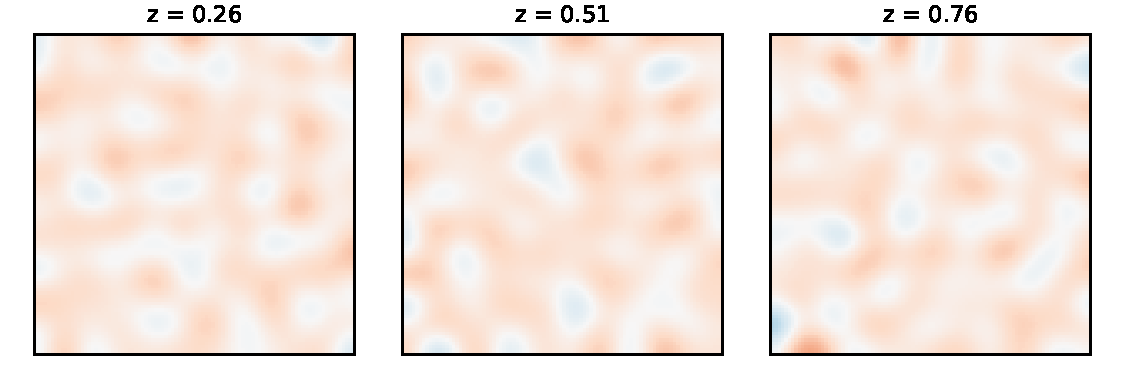
\includegraphics[width=0.62\textwidth]{cahn_hilliard_3d.pdf}
\caption{Three-dimensional Cahn--Hilliard on $96^3$: slices of the concentration at the final time.}
\end{figure}
\end{document}
